\documentclass{standalone}
\usepackage{tikz}
\begin{document}
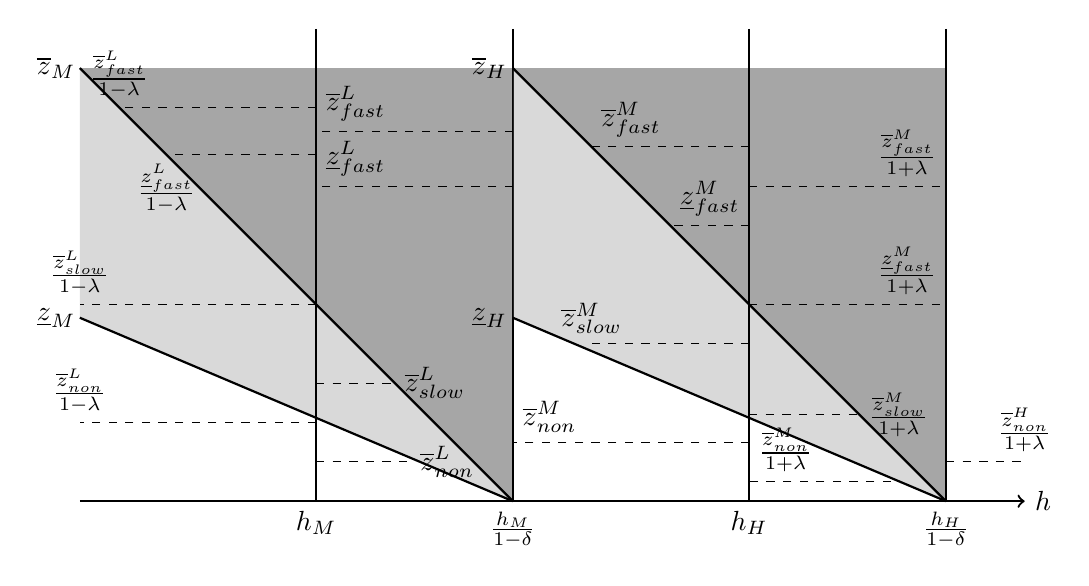
\begin{tikzpicture}


% Shaded areas (original diagram)
\fill[gray, opacity=0.3] 
    (-1,5.5) -- (4.5,0) -- (-1,2.33) -- cycle; % Top shaded region bounded by diagonals
\fill[gray, opacity=0.7] 
    (-1,5.5) -- (4.5,5.5) -- (4.5,0) -- cycle; % Bottom shaded region bounded by diagonals

% Axes for diagram
\draw[thick,->] (-1,0) -- (11,0) node[right] {$h$}; % Rescaled x-axis 

% Vertical divisions (original diagram)
\draw[thick] (2,6) -- (2,0) node[below] {$h_M$}; % Original y-axis
\draw[thick] (4.5,6) -- (4.5,0) node[below] {$\frac{h_M}{1-\delta}$}; % Vertical line for right boundary



% Diagonal lines (original diagram)
\draw[thick] (-1,5.5) -- (4.5,0); % Top diagonal line
\draw[thick] (-1,2.33) -- (4.5,0); % Bottom diagonal line





% Labels (original diagram)
\node at (-1.3,5.5) {$\overline{z}_M$};
\node at (-1.3,2.33) {$\underline{z}_M$};


% Duplicated Diagram (Starting at x = 4.5)
% Shaded areas (duplicated diagram)
\fill[gray, opacity=0.3] 
    (4.5,5.5) -- (10,0) -- (4.5,2.33) -- cycle; % Top shaded region bounded by diagonals in duplicated diagram
\fill[gray, opacity=0.7] 
    (10,5.5) -- (10,0) --(4.5,5.5) -- cycle; % Bottom shaded region bounded by diagonals in duplicated diagram
    
% Vertical divisions (duplicated diagram)
\draw[thick] (7.5,6) -- (7.5,0) node[below] {$h_H$}; % y-axis for duplicated version starting at x=7.5
\draw[thick] (10,6) -- (10,0) node[below] {$\frac{h_H}{1-\delta}$}; 

% Horizontal lines (1st region)
\draw[dashed] (2,5) -- (-0.5,5) node[above] {$\frac{\overline{z}^L_{fast}}{1-\lambda}$}; % First top dashed line
\draw[dashed] (2,4.4) -- (0.1,4.4) node[below] {$\frac{\underline{z}^L_{fast}}{1-\lambda}$}; % Second dashed line
\draw[dashed] (2,2.5) -- (-1,2.5) node[above] {$\frac{\overline{z}^L_{slow}}{1-\lambda}$}; % Third dashed line
\draw[dashed] (2,1) -- (-1,1) node[above] {$\frac{\overline{z}^L_{non}}{1-\lambda}$}; % Bottom dashed line with label

% Horizontal lines (2nd region)
\draw[dashed] (4.5,4.7) -- (2,4.7) node[above right] {$\overline{z}^L_{fast}$}; % First top dashed line
\draw[dashed] (4.5,4) -- (2,4) node[above right] {$\underline{z}^L_{fast}$}; % Second dashed line
\draw[dashed] (2,1.5) -- (3,1.5) node[right] {$\overline{z}^L_{slow}$}; % Third dashed line
\draw[dashed] (2,0.5) -- (3.2,0.5) node[right] {$\overline{z}^L_{non}$}; % Bottom dashed line with label

% Horizontal lines (3rd region)
\draw[dashed] (7.5,4.5) -- (5.5,4.5) node[above right] {\textcolor{black}{$\overline{z}^M_{fast}$}}; % First top dashed line
\draw[dashed] (7.5,3.5) -- (6.5,3.5) node[above right] {$\underline{z}^M_{fast}$}; % Second dashed line
\draw[dashed] (7.5,2) -- (5.5,2) node[above] {$\overline{z}^M_{slow}$}; % Third dashed line
\draw[dashed] (7.5,0.75) -- (4.5,0.75) node[above right] {$\overline{z}^M_{non}$}; % Bottom dashed line with label

% Horizontal lines (4th region)
\draw[dashed] (7.5,4) -- (10,4) node[above left] {$\frac{\overline{z}^M_{fast}}{1+\lambda}$}; % First top dashed line
\draw[dashed] (7.5,2.5) -- (10,2.5) node[above left] {$\frac{\underline{z}^M_{fast}}{1+\lambda}$}; % Second dashed line
\draw[dashed] (7.5,1.1) -- (8.9,1.1) node[right] {$\frac{\overline{z}^M_{slow}}{1+\lambda}$}; % Third dashed line
\draw[dashed] (9.3,0.25) -- (7.5,0.25) node[above right] {$\frac{\overline{z}^M_{non}}{1+\lambda}$}; % Bottom dashed line with label

% Horizontal lines (4th region)
\draw[dashed] (10,0.5) -- (11,0.5) node[above] {$\frac{\overline{z}^H_{non}}{1+\lambda}$}; % Bottom dashed line with label

% Diagonal lines (duplicated diagram)
% The slopes of these lines should be identical to the original version
% Top diagonal line: matching slope from (-1, 5.5) to (4.5, 0) in original diagram
\draw[thick] (4.5,5.5) -- (10,0); % Top diagonal line in duplicated version
% Bottom diagonal line: matching slope from (-1, 2.33) to (4.5, 0) in original diagram
\draw[thick] (4.5,2.33) -- (10,0); % Bottom diagonal line in duplicated version





% Labels (duplicated diagram)
\node at (4.2,5.5) {$\overline{z}_H$};
\node at (4.2,2.33) {$\underline{z}_H$};

\end{tikzpicture}



\end{document}
